\section{FAQ and Common Installation Problems}
\label{sec:faq}

\begin{comment} 

Erro de quando se abre um modelo sem ter executado a transformacao antes. Os
 ficheiros ainda n tao carregados na plataforma\ldots
 
 Solucao: adicionar atributo no modelo (nao viavel). Outra: Correr simplesmente
 a transformacao

Erro de inicializacao de prolog e isso
	Solucao: rever as path variables e copiar o jpl.jar pra lib do java. Verificar
	tbm se a versao usada do java eh a correcta.

% Erro de nome de package mal escrito.

% Erro de file not found 

% Erro de association nao declarada no metamodelo

% Erro de classe nao declarada no metamodel

\end{comment}

\subsection{SWI-Prolog: [FATAL Error: Could not find system resources]}

\emph{This error no longer occurs in the most recent version of DSLTrans.
Proceed only if you have an older version.
}

It occurs when you one (or more) of the following steps in the section \ref{sec:installation}:
\begin{itemize}
\item Install swi prolog.
\item Add the bin directory of prolog to the \emph{Path} variable.
\item Set the \emph{SWI\_HOME\_DIR} system variable.
\item Copy the jpl.jar file to the appropriate destination.
\end{itemize}

\subsection{UnsatisfiedLinkError: no jpl in java.library.path}


\emph{This error no longer occurs in the most recent version of DSLTrans.
Proceed only if you have an older version.
}

This error can be caused by many things. One of then is an incorrect \emph{PATH} \textbf{system} environment variable.
Make sure you have the following two items in your \textbf{system} \emph{PATH}:
\begin{itemize}
	\item \verb=C:\Program Files (x86)\pl\bin= (or your own path to prolog's bin
	directory);
	\item \verb=C:\Program Files (x86)\Java\jre1.8.0_25\bin= (or your own path
	to java's bin directory);
\end{itemize}

You need to restart your computer after updating the environment variable.

If this does not solve your problem, review the installation steps in the section \ref{sec:installation}.

\subsection{Prolog fatal error: EXCEPTION\_ACCESS\_VIOLATION}


\emph{This error no longer occurs in the most recent version of DSLTrans.
Proceed only if you have an older version.
}

We had this problem with the SWI-Prolog version 5.10.2 64 bits running with Java 1.7.
To solve this, you may either uninstall Java 1.7 and install java 1.6; 
or uninstall SWI-Prolog version 5.10.2 64 bits and install SWI-Prolog version 5.10.\textbf{4} 64 bits.


\subsection{ClassNotFoundException from URLClassLoader}

This exception looks like this:
\begin{verbatim}
bad class file: java\lang\
Object.class(java\lang:Object.class)
class file has wrong version 52.0, should be 50.0
Please remove or make sure it appears in 
the correct subdirectory of the classpath.
public interface ModulePackage extends EPackage {
…
loading classname: Module.ModulePackage
Error running transformation: 
C:\Users\clagms\Source Control\GitHub\
TransformationVerificationMbeddr\
EclipseProjects\MbeddrComponentLanguage
\.\transformation\mbeddr2C.dsltrans
message: ClassNotFoundException at: from: 
transformerProcessor.TransformationSource@31693a86
java.lang.ClassNotFoundException: Module.ModulePackage
	at java.net.URLClassLoader.findClass(URLClassLoader.java:381)
	at java.lang.ClassLoader.loadClass(ClassLoader.java:424)
	at java.lang.ClassLoader.loadClass(ClassLoader.java:357)
\end{verbatim}

This happens when executing the DSLTrans transformation programatically.
It is caused by the fact that you are using Java 1.8 to execute the java program that invokes the TransformerProcessor.
To solve this you need use the Java 1.6 or 1.7 to perform that execution.


\subsection{tempClasses folder does not exist}

This error happens when DSLTrans is not able to automatically create the
tempClasses folder (shown in Figure~\ref{fig:dsltrans_tempClasses}) that it uses
to generate the models runtime support code.

\begin{figure}[h]
\begin{center}
  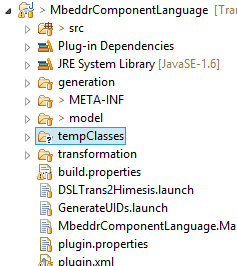
\includegraphics[width=0.6\textwidth]{imgs/dsltrans_tempClasses}
  \caption{tempClasses that DSLTrans uses as a temporary location to generate and compile code.}
  \label{fig:dsltrans_tempClasses}
\end{center}
\end{figure}

To solve this, simply create the folder.


\subsection{NoClassDefFoundError Exception IWorkspaceRunnable}

This exception looks like this:

\begin{verbatim}
Error running transformation: transformation.dsltrans
	java.lang.NoClassDefFoundError: 
org/eclipse/core/resources/IWorkspaceRunnable
	at org.eclipse.emf.codegen.ecore.genmodel.util.
		GenModelUtil.getJavaOptions(GenModelUtil.java:128)
	...
Caused by: java.lang.ClassNotFoundException: 
		org.eclipse.core.resources.IWorkspaceRunnable
	... 15 more

\end{verbatim}

It is caused when executing the DSLTrans thought the API with a missing dependency: org.eclipse.core.resources.

To solve this, go to the project that is using the DSLTrans API and add that dependency as a required package or as a required bundle, as is shown in Figure~\ref{fig:required_package_resources}.

\begin{figure}[h]
\begin{center}
  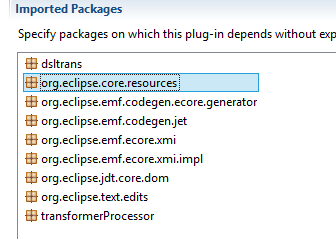
\includegraphics[width=0.6\textwidth]{imgs/required_package_resources.png}
  \caption{Missing dependency added.}
  \label{fig:required_package_resources}
\end{center}
\end{figure}





